\documentclass{article}

\usepackage[main, final]{neurips_2026}
\usepackage[utf8]{inputenc}
\usepackage[T1]{fontenc}
\usepackage{hyperref}
\usepackage{url}
\usepackage{booktabs}
\usepackage{graphicx}
\usepackage{microtype}
\usepackage{xcolor}

\graphicspath{{./}{report/DiscoveryRecommendationSkill/}}

\title{DiscoveryRecommendationSkill: Individual Report Outline}

\author{%
  Skill Author: \textit{Replace with name} \\
  Social Network Analysis, Spring 2026 \\
  \texttt{Replace with email or GitHub handle}
}

\begin{document}

\maketitle

\begin{abstract}
This outline is structured for the required three-page NeurIPS-format individual Skill report. It focuses on \texttt{DiscoveryRecommendationSkill}, the recommendation-side Skill that transforms user interest signals into arXiv query plans, candidate papers, ranked recommendations, feedback-adjusted rankings, and follow-up results. The final report should explicitly cover functionality, references, results, analysis, and visualization.
\end{abstract}

\section{Functionality}

\paragraph{Skill purpose.}
Define \texttt{DiscoveryRecommendationSkill} as the Skill responsible for finding and ranking papers before synthesis. It answers: which papers should be recommended, why are they ranked highly, and how should the recommendation adapt after seed papers or user feedback?

\paragraph{Inputs.}
List the exact input types:
\begin{itemize}
  \item \texttt{RetrievalQuery}: topic, category, date range, result budget, search mode, and query-planner mode.
  \item Seed papers: arXiv IDs, arXiv URLs, or title text used to build a \texttt{SeedPreference}.
  \item Profile state: saved seed preferences and historical like/dislike feedback.
  \item Follow-up query: local-first filters over stored papers, with optional arXiv fetch when local results are empty.
\end{itemize}

\paragraph{Outputs.}
Describe the structured outputs:
\texttt{QueryPlan}, cached \texttt{PaperMetadata}, Top-K \texttt{Recommendation} rows with rank, score, rationale, evidence label, score breakdown, feedback rank deltas, and \texttt{SkillResult} statuses for success, empty, fallback, and error cases.

\begin{figure}[t]
  \centering
  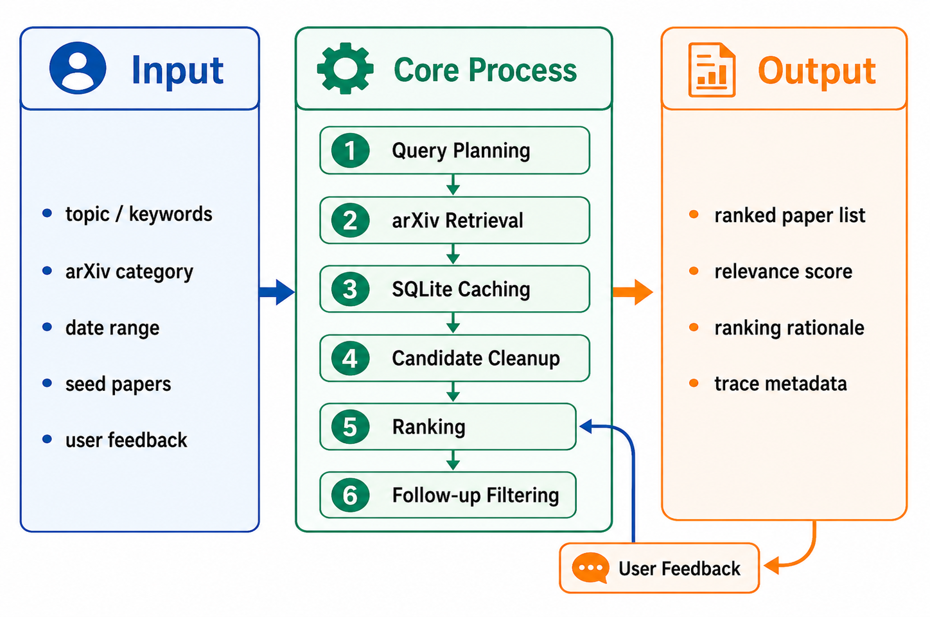
\includegraphics[width=0.88\linewidth]{skill1.png}
  \caption{Planned individual-report visualization: DiscoveryRecommendationSkill workflow from user interest signals to query planning, retrieval, ranking, feedback refinement, and follow-up filtering.}
  \label{fig:skill1-workflow}
\end{figure}

\section{Method and implementation}

\paragraph{Query planning and retrieval.}
Explain that the Skill uses a query planner to expand user input into controlled arXiv query variants. In deterministic or fallback mode, the planner preserves required terms; in live mode, invalid LLM query plans fall back to deterministic planning. Retrieval uses the arXiv Atom API, normalizes metadata, and stores papers in SQLite for cache reuse.

\paragraph{Ranking.}
Describe two ranking paths:
\begin{itemize}
  \item Deterministic ranking combines topic/query-plan matches, phrases, category/date context, seed preference, retrieval source metadata, and feedback events.
  \item Semantic seed ranking checks embedding readiness, computes seed-candidate similarity, and fails closed when real embedding credentials or seed quality are insufficient.
\end{itemize}
State that each recommendation includes a rationale so the downstream briefing can expose why a paper was selected.

\paragraph{Feedback and follow-up.}
Explain that feedback is paper-level like/dislike. The Skill records feedback events, applies latest-wins conflict handling, and returns rank/score movement after refinement. Follow-up queries search local SQLite papers first and call arXiv only when no stored papers match and fetching is allowed.

\section{References and related work}

Use this section to ground the Skill in information retrieval and recommender-system methods:
\begin{itemize}
  \item arXiv API retrieval as the source of scholarly metadata \citep{arxivapi}.
  \item Classical information retrieval and ranked retrieval metrics such as precision, recall, and MRR \citep{manning2008}.
  \item Hybrid content-based recommendation for combining topic, category, seed, and feedback signals \citep{burke2002}.
  \item Sentence embedding similarity for semantic seed recommendation \citep{reimers2019}.
\end{itemize}

\section{Results}

Report deterministic offline results from the search-quality fixture and the Unit 8 evaluation helpers. Make clear that the goal is repeatable Skill validation, not a large-scale benchmark claim.

\begin{table}[t]
  \centering
  \caption{Planned DiscoveryRecommendationSkill results table.}
  \label{tab:skill1-results}
  \begin{tabular}{lll}
    \toprule
    Evaluation & Metric & Fixture-backed result \\
    \midrule
    Broad planned search & relevant candidate coverage & 1.0 \\
    Top-K ranking & precision@3 / recall@3 / MRR & 1.0 / 1.0 / 1.0 \\
    Explanation support & rationale coverage & 1.0 \\
    Semantic seed ablation & lexical baseline precision@K & 0.0 \\
    Semantic seed ablation & semantic precision@K & 1.0 \\
    Feedback refinement & reported output & rank and score movement \\
    \bottomrule
  \end{tabular}
\end{table}

\paragraph{Qualitative demo results.}
Use the presentation example: with topic ``world model'' and seed papers about ``world action model,'' the recommendations concentrate on robotics-related world-model papers. In the profile-only demo, historical seed papers and feedback drive recommendations toward robotics and deep learning without a fresh topic.

\section{Analysis}

\paragraph{What works and why.}
Argue that broad query planning improves candidate recall over strict phrase retrieval; seed papers and semantic similarity make recommendations more personalized; rationales and score breakdowns make ranking inspectable; feedback refinement gives users visible control; and local-first follow-up makes interaction faster and more contextual.

\paragraph{Ablations and failure cases.}
Include the following analyses in the final report:
\begin{itemize}
  \item Strict phrase retrieval versus broad planned retrieval.
  \item Lexical-only baseline versus semantic seed ranking.
  \item Before/after feedback movement for liked and disliked papers.
  \item Local follow-up hit versus empty local store with optional fetch.
\end{itemize}
Discuss failure behavior: invalid query plans fall back, empty retrieval returns structured empty results, semantic mode fails closed, and provider payloads or raw vectors are not exposed in traces.

\section{Page allocation for the final three-page report}

\begin{table}[h]
  \centering
  \caption{Suggested three-page allocation. References do not count toward the page limit.}
  \label{tab:skill1-page-plan}
  \begin{tabular}{ll}
    \toprule
    Page target & Content \\
    \midrule
    Page 1 & Functionality, inputs/outputs, Figure~\ref{fig:skill1-workflow} \\
    Page 2 & Method, implementation details, related work \\
    Page 3 & Results, ablations, limitations, StudyClawHub metadata \\
    \bottomrule
  \end{tabular}
\end{table}

\section*{Checklist before finalizing}

\begin{itemize}
  \item Replace author placeholders and add the published StudyClawHub Skill URL.
  \item Keep the final individual report at three pages before references.
  \item Include at least one visualization; Figure~\ref{fig:skill1-workflow} satisfies the requirement.
  \item Keep recommendation evidence separate from abstract/full-text evidence.
\end{itemize}

\begin{thebibliography}{9}

\bibitem[arXiv(2026)]{arxivapi}
arXiv.
\newblock arXiv API User Manual.
\newblock \url{https://info.arxiv.org/help/api/index.html}.

\bibitem[Burke(2002)]{burke2002}
Robin Burke.
\newblock Hybrid recommender systems: Survey and experiments.
\newblock \emph{User Modeling and User-Adapted Interaction}, 12:331--370, 2002.

\bibitem[Manning et~al.(2008)]{manning2008}
Christopher D. Manning, Prabhakar Raghavan, and Hinrich Schutze.
\newblock \emph{Introduction to Information Retrieval}.
\newblock Cambridge University Press, 2008.

\bibitem[Reimers and Gurevych(2019)]{reimers2019}
Nils Reimers and Iryna Gurevych.
\newblock Sentence-BERT: Sentence embeddings using Siamese BERT-networks.
\newblock \emph{EMNLP-IJCNLP}, 2019.

\end{thebibliography}

\end{document}
